\documentclass{article}

\usepackage{tikz,lipsum,lmodern}
\usepackage[english]{babel}
\usepackage[most]{tcolorbox}
\usepackage[paperheight=10.75in,paperwidth=7.25in,margin=1in,heightrounded]{geometry}
\usepackage{graphicx}
\usepackage{blindtext}
\usepackage{ragged2e}
\usepackage{needspace}
\usepackage[space]{grffile}
\usepackage[utf8]{inputenc}
\usepackage[export]{adjustbox}
\usepackage{hyperref}
\usepackage{placeins}
\usepackage{xcolor}
\usepackage{float}
\usepackage{fancyhdr}

\pagestyle{fancy}
\fancyhf{}
\rhead{\rightmark}
\chead{\thepart}
\lhead{\nouppercase{\leftmark}}
\cfoot{\thepage}
\graphicspath{{"./img/"}}

\hypersetup{
    colorlinks,
    citecolor=black,
    filecolor=black,
    linkcolor=black,
    urlcolor=black
}

\graphicspath{{"./img/"}}



\begin{document}

\section{section}
\subsection{subsection}


\begin{figure}[H]
	\centering
	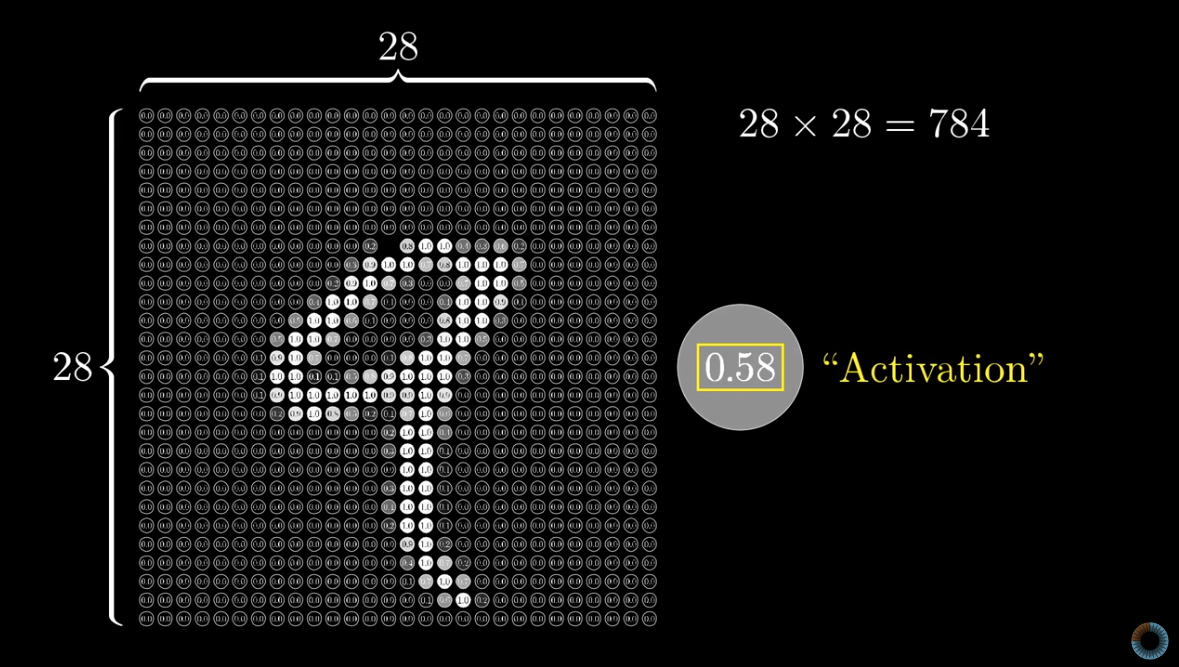
\includegraphics{ai_1.png}
	\caption{test}
	\label{testlabel}
\end{figure}

\begin{figure}[H]
	\centering
	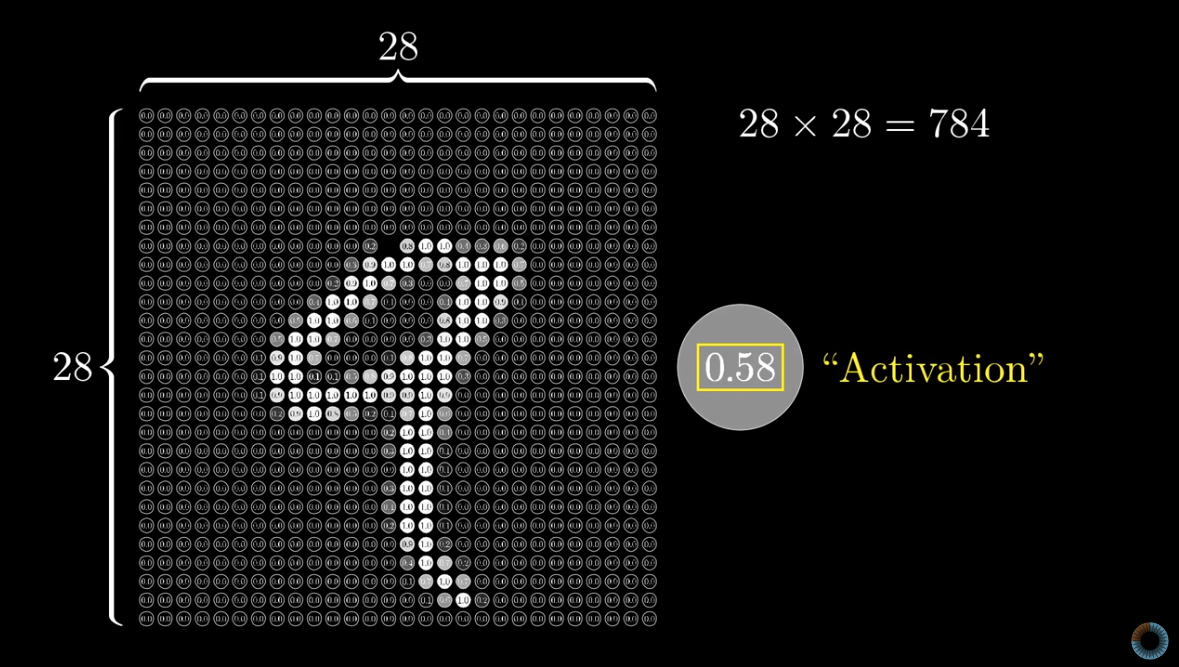
\includegraphics{ai_1.png}
	\caption{test2}
	\label{testlabel2}
\end{figure}

test test \ref{testlabel2}

\end{document}
